% TODO: How data are stored? Storage - structured, unstructured, semi-structured
% Naming convention Data format

\subsection{Data modeling}
In developing a comprehensive software system, it's crucial to approach data
modeling with a structured and strategic framework that encompasses various
aspects of the application's functionality and security. To provide a clear and
logical understanding of this framework, we will explore three critical models
that collectively define the architecture of modern software systems:
core model, identity model, and form model. Each model serves a distinct purpose and
complements the others, ensuring a robust, secure, and user-friendly
application. Let's delve into these models in the order that mirrors their
integration and importance in the development process.

We begin with the core model, the backbone of our application. This model is
where the fundamental business logic and core data structures are established.
It defines the essential entities and their relationships that form the basis of
the system, focusing on how data is organized and manipulated to support the
application’s primary services and functionalities. By starting with core model,
we set the groundwork for all other aspects of the system, highlighting the
primary operations and data flows that are crucial for the application's
purpose.
\begin{figure}[H]
  \centering
  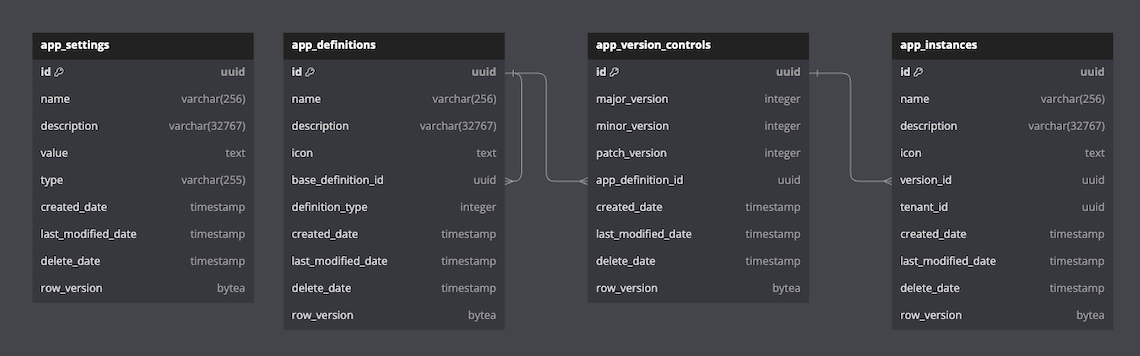
\includegraphics[width=\linewidth]{Images/model_core.png}
  \vspace{1em}
  \caption{The Core Model}
\end{figure}

Once the core functionalities are established, we shift our focus to security
with the identity model. This model is dedicated to managing user authentication and
authorization. It ensures that access to the information and functionalities
defined in core model is securely controlled. By integrating Identity model, we
discuss how the system protects sensitive data and operations from unauthorized
access, ensuring that users can interact with the core components in a secure
environment. This model not only reinforces the security of the system but also
defines user roles and permissions, which are essential for a multi-user
application. 
\begin{figure}[H]
  \centering
  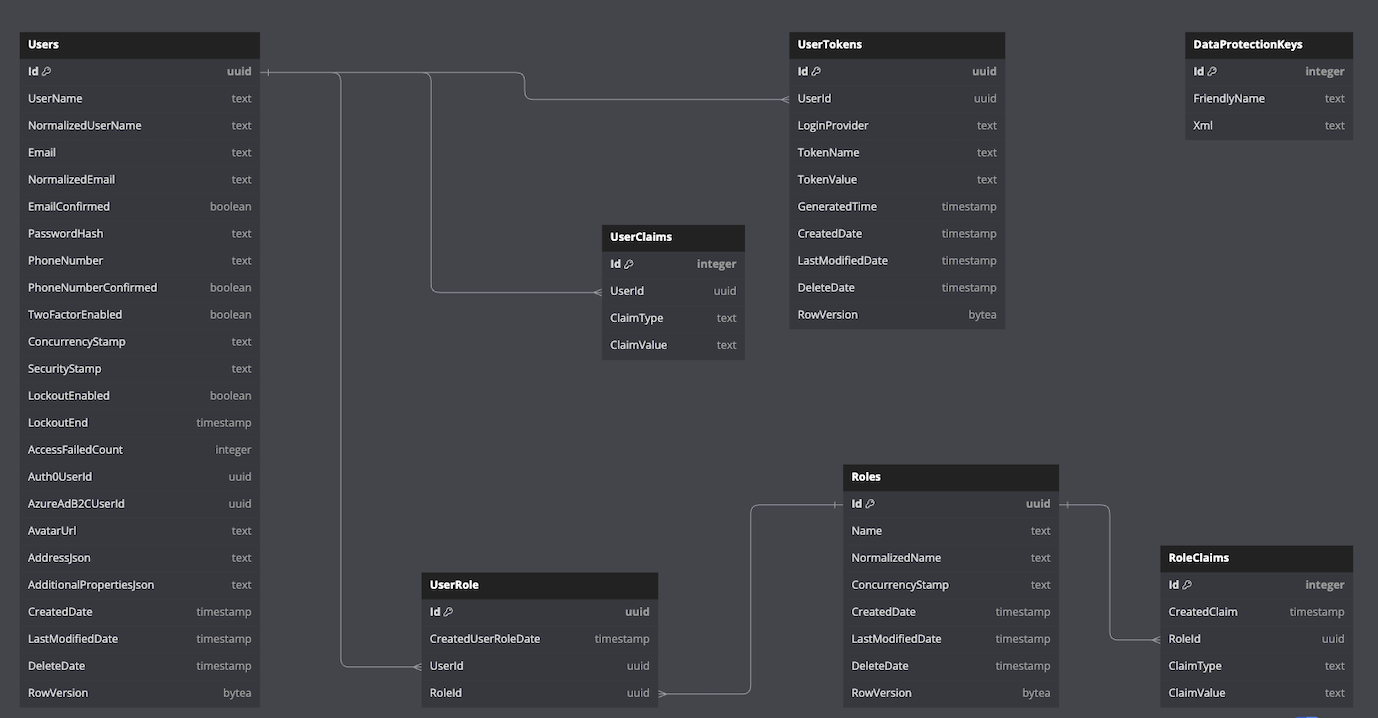
\includegraphics[width=\linewidth]{Images/model_auth.png}
  \vspace{1em}
  \caption{The Identity Model}
\end{figure}

Finally, we explore the form model, which ties the user interface and
interaction directly to the underlying data structures of the core model and the
security protocols of the Identity model. This model addresses how users will
experience and interact with the application through various forms and
interfaces. It encompasses everything from data entry and management to ensuring
that user interactions are intuitive and efficient. form model is critical for
defining the presentation and accessibility of the system’s features, making
sure that the application is not only functional and secure but also
user-friendly and responsive to the needs of its users.
\begin{figure}[H]
  \centering
  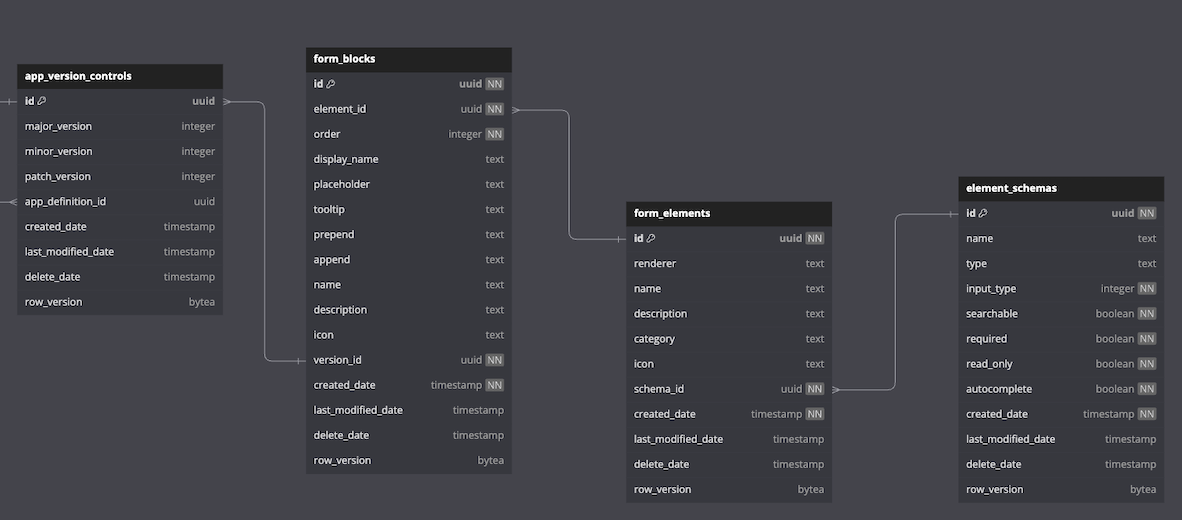
\includegraphics[width=\linewidth]{Images/model_form.png}
  \vspace{1em}
  \caption{The Form Model}
\end{figure}

By examining these models in this order, we effectively build from the internal
architecture to the external user interface, providing a comprehensive view of
the system's design from the ground up. This approach helps in understanding how
each component is interlinked and why each is vital to the overall success and
operability of the application.
\subsection{Blob storage}
As an intermediary entity situated between the data producers, exemplified by
the radar center, and the data consumers, represented by the Data Model and
Machine Learning team, our paramount responsibility lies in ensuring that the
data management infrastructure is meticulously designed to seamlessly
accommodate the diverse and often contrasting requirements set forth by both
parties.

The dataset, procured from the esteemed Nha Be radar center, adheres to the
rigorous SIGMET format, as delineated in \ref{sigmet}. This format encompasses a
plethora of scalar values pertaining to metadata facets such as the radar's
nomenclature, the modality of scanning employed, and the temporal stamp denoting
the execution of the scan. Concurrently, this data corpus embodies a rich array
of multidimensional metrics encapsulating various meteorological phenomena,
including but not limited to reflectivity and energy profiles.

Collaborative engagements with the modeling cadre, predominantly comprising
members from the distinguished teams led by Tu and Vinh, have endowed us with a
nuanced understanding of their exigencies and prerequisites vis-à-vis data
structuring paradigms. From the purview of these erudite teams, data
representation assumes two principal manifestations. Firstly, there is a
pronounced inclination towards encapsulating data in the form of images tailored
to specific geographical demarcations within the Vietnamese domain. A
quintessential exemplar of this utilization paradigm is elucidated in Figure
\ref{fig:nha-be-viz-far}, which encapsulates the data instrumental in honing the
multimodal solutions. Alternatively, there exists a proclivity towards direct
data consumption in the form of NumPy Tensors, leveraging the expansive spectrum
of NumPy-compatible APIs inclusive of those furnished by SciPy and XArray.
Although ostensibly more efficient, this mode of data consumption has not
garnered widespread adoption within the precincts of our collaborative endeavor.

Armed with an exhaustive comprehension of the requisites delineated by both
stakeholders and guided by heuristic principles germane to the architecture of
rudimentary data warehousing systems, we proffer a set of salient properties
that our envisaged system ought to embody:

Primarily, the envisaged data repository must find its abode in an Object
Storage medium, characterized by maximal interoperability with extant systems.
This necessitates the exclusion of proprietary solutions such as Google Cloud
Storage or Azure Storage Blob in favor of alternatives such as Hadoop
Distributed File System (HDFS) \cite{HDFS} or any Object Storage infrastructure
compliant with AWS S3 protocols. While HDFS presents itself as a viable
candidate, the logistical intricacies entailed in deploying and administering a
comprehensive HDFS cluster militate against prioritizing its adoption.
Fortuitously, our discerning team has identified a panacea in the form of MinIO,
an open-source Object Storage solution that not only aligns with the requisites
of our project but also boasts compatibility with prevailing AWS S3 APIs.

The conundrum surrounding the optimal data format to be stored within the Object
Storage reservoir has been a subject of fervent debate and contention amongst
our learned colleagues. While proponents of denormalization advocate for its
adoption to streamline data retrieval processes, empirical evidence underscores
the efficacy of the RAW data format in compressing and storing multidimensional
datasets, as attested by the diminutive file sizes characteristic of individual
scan executions. Indeed, attempts to transmute this format into alternative
structures, such as JSON, have yielded negligible dividends owing to the
intrinsic complexity of the dataset. Moreover, with the ascendancy of multimodal
Machine Learning paradigms, necessitating the simultaneous retrieval of diverse
data fields to facilitate batch processing, the retention of all pertinent
fields within a singular RAW file emerges as a prescient strategy poised to
accommodate the evolutionary trajectory of our modeling endeavors.

In delineating a nomenclatural schema for the files ensconced within the Object
Storage repository, precedence is accorded to a rudimentary ordering scheme
premised on tenant identification and temporal demarcation. For the myriad
utilization scenarios contemplated heretofore, the concatenation of the tenant
identifier with a timestamp proves to be a judicious nomenclatural convention.
Furthermore, the hierarchical organization of files within the Object Storage
framework ought to be predicated on a delineation between tenant-specific
directories and temporal partitions.

Regarding the temporal component of the nomenclatural schema, adherence to the
ISO-8601 standard, a globally ratified temporal convention, is deemed
imperative. The employment of the ISO-8601 timestamp format, typified by the
concatenation of year, month, day, hour, minute, and second components devoid of
any superfluous delimiters, serves to obviate compatibility issues with extant
filesystems. Notably, the conspicuous absence of special characters such as
hyphens and colons serves to circumvent prohibitions imposed by certain
filesystems, such as Windows, on the usage of such characters within filenames.
